\chapter{Design And Implementation} % - Design and Implementation
\label{chap:design}
%   - overview
%   - original tinkering and considerations
%   - features and considerations
%       - readline
%       - golang
%       - logging
%           - remote phoning home
%       - extensibility (markdown, parser)
%       - embedded files
%           - Template expansion
%           - Running examples
%       - usability 
%   - architecture of cli-tool
%   - architecture of web-tool
%       - how sandboxing is achieved

%docker deamon exposed over https for the sake of websockets. something the sdk cannot handle.

\section{Tools and Libraries}
\label{sec:tools}

\subsection{\textit{CLI-Tutor}}
\begin{itemize}
    \item \textit{readline} is the \textit{Go} port of the gnu readline
        \cite{ramey_fox_readline} line editing software. It forms the backbone
        of the lesson menu in \textit{CLI-Tutor}.

    \item \textit{bubbletea} is \textit{Go} framework for building stateful terminal
        applications using the Elm Architecture\footnote{More on the Elm
        Architecture here: \url{https://guide.elm-lang.org/architecture/}}.
        \textit{bubbletea} is a part of the charm\footnote{More on the charm
        project here: \url{https://charm.sh}} project, which is a host of
        frameworks and libraries aimed at modernising the command line
        interface. The project also includes a host of smaller libraries and
        extensions designed to be used with \textit{bubbletea}
        applications.\textit{bubbletea} is the tui framework used to manage
        switching between the menu and lesson views in \textit{CLI-Tutor}.

        \begin{itemize}
            \item \textit{bubbles} is a collection of ui components to be used alongside \textit{bubbletea}.
            \item \textit{bubblezone} is a community contributed extension to
                \textit{bubbles} components that allows for zones and hit boxes
                to be established in the user interface.
            \item \textit{lipgloss} is a styling and layout toolkit for \textit{bubbletea} applications.
        \end{itemize}

    \item \textit{glamour} is a terminal Markdown rendering library also
        created by the \textit{charm} team. It is used to display lesson tasks
        during a lesson in \textit{CLI-Tutor}.

    \item \textit{cobra} is a very popular CLI framework that is used in
        \textit{CLI-Tutor} for feature flags, the help menu and for managing
        start up and clean up behaviours.
        
    \item \textit{goldmark} is a Markdown parser written in \textit{Go}. It is used in
        \textit{CLI-Tutor} for parsing lesson files into data structures that
        drive the lesson interface and also for populating the menu with a list
        of available lessons.

    \item \textit{termenv}  is a \textit{Go} library used for managing terminal colours
        and environments. It is used in \textit{CLI-Tutor} for maximising
        compatibility across terminals, producing colours and for certain
        terminal controls such as screen clearing.
\end{itemize}

\subsection{Web Application}
\begin{itemize}
    \item \textit{Svelte} is a JavaScript/TypeScript frontend framework. It was
        chosen to be the frontend for our web application due to its
        simplicity, low learning curve and bundled output approach.

    \item \textit{Vite} is the JavaScript bundler used alongside Svelte to package the project for the web.

    \item \textit{XtermJs} is a terminal component for frontend applications.
        It is famously used as the terminal in the extremely popular text
        editor VSCode\footnote{More about VSCode here:
        \url{https://code.visualstudio.com/}}. The terminal component is used
        alongside it's \textit{attach} add-on to form a connection over
        WebSockets to a \textit{docker} container. This is how sandboxed environments
        are provided over the web to users.

    \item \textit{Fiber} is the HTTP framework used to create the backend for
        our web application. It is primarily used as a proxy between the
        frontend and the \textit{docker deamon} running on our backend server.

    \item \textit{Docker SDK} is a first party \textit{Go} Software Development Kit
        (SDK) for interacting with the \textit{docker deamon}. It was chosen for
        interoperability with the backend HTTP framework which also uses \textit{Go}.

    \item \textit{MkDocs} is an industry standard static site generator for
        documentation websites. It was used to create a documentation website
        for the user study conducted in this work.
        \begin{itemize}
            \item \textit{MkDocs-Material} is an extension to \textit{MkDocs}
                providing an attractive modern theme and some additional visual
                elements to the static documentation website created for
                \textit{CLI-Tutor}.
        \end{itemize}
\end{itemize}

\subsection{Server Infrastructure}
\begin{itemize}
    \item \textit{Linode} is a cloud service provider offering low cost Virtual Private Servers. Two servers were used to implement the web application portion of \textit{CLI-Tutor}.
    \item \textit{Nginx} is a high performance web server. It was utilised on
        both our servers to serve as a reverse proxy to allow communication
        with \textit{docker} and our backend API.
    \item \textit{Gitlab CI/CD} is a Continuous Integration and Continue Delivery service used for testing, building and deploying our web application.
    \item \textit{Grafana Cloud} is a monitoring service. It was used in
        \textit{CLI-Tutor} to monitor uptime and for log agglomeration from our
        servers to ensure everything was running well.
\end{itemize}

\section{First Attempts} In the early stags of this thesis work, while
attempting to model the problem and develop the requirements for a technical
solution a number of prototypes were created. The early prototypes were written
in \textit{Python} \cite{python}. It was clear from an early stage that
\textit{readline} would be a mandatory element of approach we would take. Early
attempts broadly focused on two different approaches:

\begin{itemize} \item An \textit{Expect}\cite{libes1995exploring} like
    approach. \textit{Expect} is an add-on to the \textit{Tcl} scripting
    language and is a way of writing scripted interactions with sub processes.
    An \textit{Expect} script can be used to launch a sub process and
    communicate with it, for each action expected results can be specified.
    \textit{Expect} scripts are popular for feigning user input and for testing
    or combining separate services. It is designed entirely with command line
    applications in mind and thus seemed a worthwhile approach for
    \textit{CLI-Tutor}, especially because we wanted to design lessons which
    had expected values and interactive exercises. Two prototypes were build
    using  \textit{Python} and \textit{Go}. The plan was to use \textit{Expect}
    to interact with a spawned \textit{Bash} sub process. While initially
    promising, the \textit{Expect} approach was abandoned due to limitations in
    the libraries and concerns around being able to building an appropriate
    user interface to wrap \textit{Expect}.

    \item Creating and managing PTYs\footnote{PTY refers to a Linux
        psuedoterminal, the low level interface through which terminal data
    flow is implemented in Linux.}. Prototypes integrating \textit{readline}
    implementations were built using this approach with some success. However,
    this approach necessitated intricate low level programming and raw
    communication with the terminal. It was eventually deemed too complicated
    and operating system specific to be appropriate for the purpose of
    \textit{CLI-Tutor}. \end{itemize}

    Other attempts included writing a GUI application to create a fake terminal
    environment. However, it was decided that a compiled command line
    application would be most appropriate for this purpose as it would allow us
    to capitalise on the existing interface of the user's terminal and the
    wealth of libraries and tools available to facilitate command line
    application development. An approach of creating a mock shell environment
    and using operating system native system calls would be the most proper
    approach for \textit{CLI-Tutor}.

\section{Features and Considerations of \textit{CLI-Tutor}}

\subsection{Why \textit{Go}?} The \textit{Go} programming language was selected
for \textit{CLI-Tutor} for numerous reasons. \textit{Go} is a popular language
for writing command line applications, with numerous modern CLI applications
such as the \textit{GitHub} CLI \cite{github_cli} and \textit{docker} CLI
\cite{dockerinc_2022}. This popularity in CLI applications also has the side
effect of there being a wide selection of libraries available for implementing
CLI interfaces (see: \autoref{sec:tools}). In addition to good tooling,
\textit{Go} programs are compiled and this easier to distribute across
operating systems than interpreted alternatives such as \textit{Python}
programs. 


\subsection{Shell environment}

\subsection{Lessons}

\subsubsection{Anatomy of a Lesson} A lesson is a container that contains a
series of tasks. A lesson has a title and description which are used to
populate the menu screen of \textit{CLI-Tutor}. Every task contains a title and
description as well. The title of a task is displayed in the task tracker and
the description is the actual textual content of a task. This content is either
explaining a concept to the user, displaying a diagram or prompting the user to
input some commands. The amount of tasks dictates the length of the lesson. The
user can keep track of their progress inside a lesson by the task tracker,
which displays the title of the current task as well as a progression counter.

\vspace{1em}
\begin{lstlisting}[frame=single, caption=Data structures for a Lesson and a Task within a Lesson.]
type Lesson struct {
	Name        string
	Vocabulary  []string
	Description string
	Tasks       []Task
}

type Task struct {
	Title       string
	Description string
	Expected    string
}
\end{lstlisting}

\subsection{Embedded Files}
\subsubsection{Template Expansion}
\subsubsection{Running Examples}

\subsection{Usability}

\subsection{Logging}

%talk more about the data structures here 

\section{Web Application}

\subsection{Overview of Web Application}

\paragraph{Frontend} The frontend is a simple Javascript web application that
presents the user with a special front end terminal component. This component
is then connected to a backend API\footnote{Application Programming Interface}
running on the same server which uses \textit{docker} to create containers on
demand. The containers are then connected to the web terminal (see: \autoref{fig:webversion}) on the frontend
and a WebSocket\footnote{A full-duplex communication protocol native to modern
web browsers.} connection is established to allow the user to interact
with the provisioned \textit{docker} container.

\paragraph{Backend} The backend is a REST\footnote{Representational state
transfer: An architectural style for creating interfaces to allow Client-Server
communication.} API, written in \textit{Go}. The API allows the frontend to communicate
with the \textit{docker daemon} running on the server, to create,
resize and stop containers on the backend.
 
\paragraph{CLI Only} As mentioned earlier, a CLI only version (see: \autoref{fig:cliversion})was also created
using essentially the same architecture as the version that includes
\textit{CLI-Tutor}. Slight visual differences were made to differentiate the
two however they are based on fundamentally the same \textit{docker} image, with
the only difference being that the "CLI Only" version does not contain the
\textit{CLI-Tutor} tool and drops the user directly into a Linux shell.

\paragraph{Documentation Website} Created using MkDocs,\cite{mkdocs} a widely
used tool for documentation in the software development world. The
documentation website (see: \autoref{fig:docsweb}) was also built to support the
User Study. It uses the same lessons as in the \textit{CLI-Tutor}
application, albeit with some prompts for user interface actions removed.

\paragraph{Logging} To assist with gathering usage data and user behaviour,
\textit{CLI-Tutor} maintains a log file which can be optionally sent back to a
server for examination. The log file is a mirror copy of the lesson session
with timestamps for every action that occurs during the lesson.

\section{Architecture}

\subsubsection{Anatomy of a lesson} A lesson is a container that contains a
series of tasks. A lesson has a title and description which are used to
populate the menu screen of \textit{CLI-Tutor}. Every task contains a title and
description as well. The title of a task is displayed in the task tracker and
the description is the actual textual content of a task. This content is either
explaining a concept to the user, displaying a diagram or prompting the user to
input some commands. The amount of tasks dictates the length of the lesson. The
user can keep track of their progress inside a lesson by the task tracker,
which displays the title of the current task as well as a progression counter.

\section{Extending CLI-Tutor}

\begin{lstlisting}[float=htbp, frame=single, language={}, label=lst:markdown, caption=Specification for Markdown lesson files.]
# Lesson Title

A line under a level 1 heading is the lesson description. This is also
displayed in the menu.

## First Task Title

Task instructions are parsed as normal lines under a level 2 heading.

Even line breaks and nested elements will reflect in the lesson. This greatly
enhances readability.

`Commands` are highlighted with backticks.

Text can be injected into a lesson at the time of parsing with template
functions like this --> {{SomeFunc}}

## Second Task Title

This is the first line following a second level 2 heading and thus the text of
task #2.

```
Code blocks can also be used to represent larger blocks of instructions or for
ASCII diagrams.
```
## Interactive tasks with expected values

If the current task is expecting a certain output to a command the user types,
we can specify that using the `>` syntax.

> {{TestFunc}}

## Runtime expected value calculation

Sometimes the correct value for a given task can only be computed at run time,
to achieve this we can specify the expected value of a task to be the output of
a system call by prepending a `!` and then the expected command.

> !ls -la

### Lesson Vocabulary (Provided as a comma separated list of values under a
level 3 heading )

vim, ls, cp, cat, echo <--- only these commands will be permitted in this lesson.

\end{lstlisting}

\begin{figure}[htbp]
	\centering
	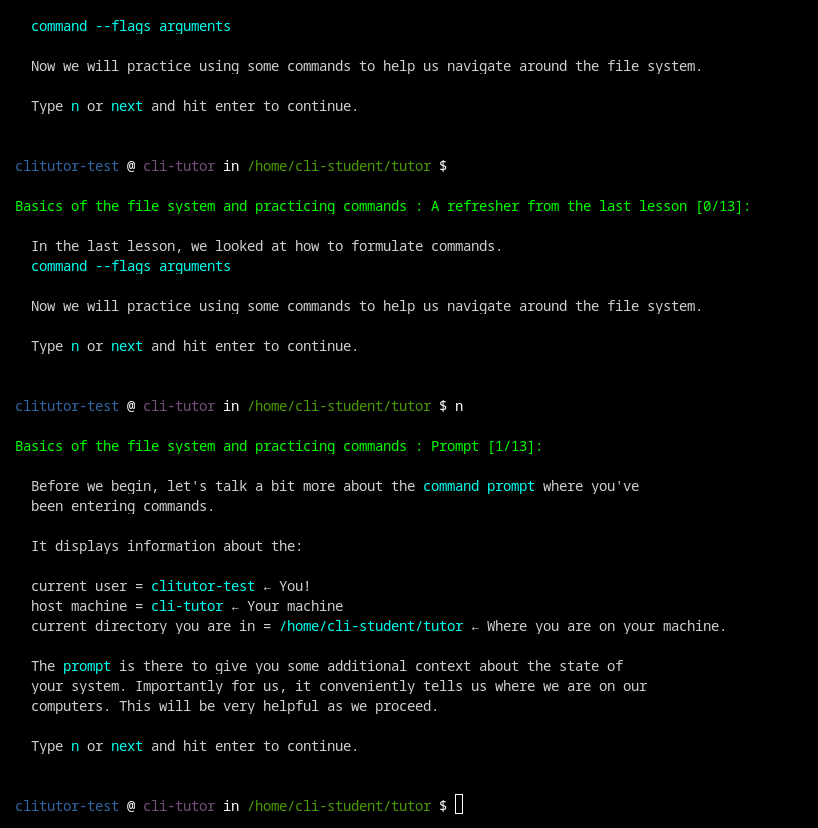
\includegraphics[width=1\textwidth]{img/cliexpansionfull}
	\caption{Screen shot of a \textit{CLI-Tutor} lesson showing values interpolated into the lesson.}
	\label{fig:templateexpansion}
\end{figure}
